\Chapter{Implementatie}\label{hfdst-implementatie}

In dit hoofdstuk wordt de implementatie van een schakeling voor de berekening van de Tate pairing uit de doeken gedaan. Er zal onderzocht worden welke basisbewerkingen nodig zijn en hoe deze verwezenlijkt kunnen worden in hardware. Vervolgens wordt een schakeling ontworpen die aan de hand hiervan alle nodige berekeningen kan uitvoeren in het veld $\mathbb{F}_{2^m}$. Ten slotte is er dan nog de schakeling die alle berekeningen voor het Miller algoritme in goede banen leidt. Allereerst wordt echter gekeken welke beperkingen aan de implementatie opgelegd moeten worden.

\section{Beperkingen}\label{sectie-implementatie-beperkingen}

Het doel is de uiteindelijke schakeling zo klein mogelijk te maken, zodat ze gebruikt kan worden in bv.\ netwerken van sensoren of smartcards. Beperking van de oppervlakte is dus de belangrijkste factor. Een tweede belangrijke factor is stroomverbruik, maar dat is helaas zeer moeilijk te berekenen. Het verbruik hangt echter samen met de oppervlakte, dus het beperken daarvan zal ook het verbruik ten goede komen. Het verbruik kan ook verlaagd worden door een lagere kloksnelheid voor de schakeling te gebruiken, wat uiteraard de rekensnelheid niet bevordert. De rekensnelheid is echter geen prioriteit en dus kan dit aspect bij het ontwerp van de schakelingen genegeerd worden. Op dit alles zal dieper ingegaan worden in \refhfdst{hfdst-resultaten}

Algemeen kan gesteld worden dat hoe kleiner het uiteindelijke resultaat is, hoe beter. Het is dus cruciaal de elementen te identificeren die het meeste plaats innemen in een ASIC schakeling. In \reftbl{tabel-implementatie-beperkingen-elementen-gatecount} is de grootte van de belangrijkste elementen te vinden. Deze cijfers gelden enkel bij gebruik van $0.13 nm$ low leakage technologie. De ordening van de elementen blijft echter behouden voor andere technologi\"en. Uit de tabel blijkt dat het gebruik van flip-flops (registers), adders en multiplexers zoveel mogelijk beperkt moet worden.

\begin{table}[h]
	\caption{Grootte van elementen in een ASIC schakeling in gates$/$bit ($0.13 nm$ low leakage technologie)\cite{cell-databook}}
	\label{tabel-implementatie-beperkingen-elementen-gatecount}
	\begin{tabular}{|l|r|}
		\hline
		Element			& Gates$/$bit\\
		\hline
		D flip-flop met reset	& 6\\
		D flip-flop zonder reset	& 5.5\\
		D latch			& 4.25\\
		full adder		& 5.5\\
		3 ingang MUX	& 4\\
		2 ingang XNOR	& 3.75\\
		2 ingang XOR	& 3.75\\
		2 ingang MUX	& 2.25\\
		2 ingang OR		& 1.25\\
		2 ingang AND	& 1.25\\
		2 ingang NOR	& 1\\
		2 ingang NAND	& 1\\
		NOT				& 0.75\\
		\hline		
	\end{tabular}
\end{table}

\section{Modular Arithmetic Logical Unit}\label{sectie-implementatie-malu}

De kern van de hardware implementatie wordt gevormd door de Modular Arithmetic Logical Unit (MALU)\cite{sakiyama}. Dit circuit laat toe basis bewerkingen uit te voeren op getallen. Gezien de beperking die is opgelegd aan de oppervlakte van de schakeling, wordt enkel de optelling ge\"implementeerd. Later wordt met behulp daarvan elke andere nodige berekening verwezenlijkt.

Aangezien er in het veld $\mathbb{F}_{2^m}$ gewerkt wordt, is een optelling equivalent aan een XOR bewerking. De bewerking die moet uitgevoerd kunnen worden is:

\[\begin{aligned}
T + B	&= T \xor B\\
		&= R \mod P
\end{aligned}\]

Merk op dat bij een optelling de graad van $R$ enkel kleiner of gelijk kan zijn aan die van $T$ en $B$. Indien $B$ van graad $\leq m$ is en $T$ van graad $\leq m + 1$, is de modulo bewerking te implementeren als in \refalg{algoritme-implementatie-malu-modulo}.

\begin{algorithm}[h]
\caption{Modulo optelling in $\mathbb{F}_{2^m}$}
\label{algoritme-implementatie-malu-modulo}
	\KwIn{$B \in \mathbb{F}_{2^m}$, $T \in \mathbb{F}_{2^{m + 1}}$}
	\KwOut{$R \mod P \in \mathbb{F}_{2^m}$}
	\SetKwFunction{Degree}{Degree}

	$R \leftarrow T \xor B$\;

	\If{$\Degree{T} = m$}{
		$R \leftarrow R \xor P$\;
	}
\end{algorithm}

Een voor de hand liggende schakeling die dit alles implementeert, is te zien in \reffig{figuur-implementatie-malu-basic-noshift}. Ingang $P_{\text{in}}$ dient afhankelijk van $T_{m}$ ingesteld te worden op $0$ of $P$. $P_{m}$ kan genegeerd worden, aangezien in het resultaat de graad $< m$ is.

\begin{figure}[h]
	\begin{center}
		\includegraphics[width=12cm]{malu-basic-noshift}
		\figcaption{MALU - Basis ontwerp}\label{figuur-implementatie-malu-basic-noshift}
	\end{center}
\end{figure}

In \refsect{sectie-implementatie-gf2m} zal blijken dat het vaak nodig zal zijn om het resultaat $R$ te vermenigvuldigen met $z$, maw.\ alle bits 1 plaats naar links te verschuiven. Indien die bewerking wordt toegevoegd, bekomt men de schakeling uit \reffig{figuur-implementatie-malu-basic}. Net als de vorige implementatie bestaat deze uit $2m$ XOR poorten.

\begin{figure}[h]
	\begin{center}
		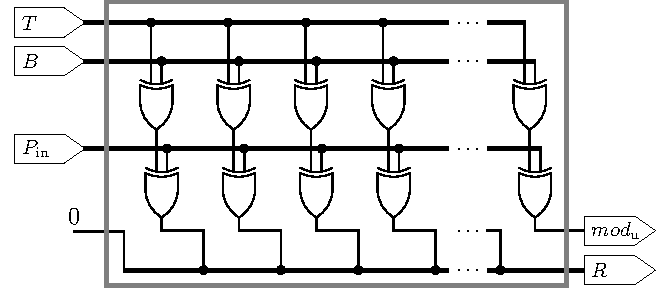
\includegraphics[width=12cm]{malu-basic}
		\figcaption{MALU - Basis ontwerp met shift}\label{figuur-implementatie-malu-basic}
	\end{center}
\end{figure}

Aangezien voor het ontwerp het veld en de modulo veelterm op voorhand bepaald zijn, is het mogelijk een zeer groot aantal XOR poorten uit het ontwerp te verwijderen. De ingang en de bijhorende $m$ XOR poorten kunnen vervangen worden door een 1 bit `modulo enable' ingang $mod_{\text{in}}$ en er worden enkel XOR poorten geplaatst voor de bits $i$ waarvoor $P_i = 1$. Hierdoor wordt het aantal ingangen drastisch verkleind en worden 
\[\Delta = m - (\text{hamm}(P) - 1)\]
XOR poorten uitgespaard, met hamm$(P)$ gelijk aan het Hamming gewicht van de binaire representatie van $P$.

In dit geval is $m = 163$ en $P = z^{163} + z^7 + z^6 + z^3 + 1$. Er zijn dus $\text{hamm}(P) - 1 = 4$ XOR poorten nodig, wat een besparing van $163 - 4 =  159$ XOR poorten oplevert ($51\%$ kleiner dan de oorsponkelijke grootte).

De resulterende schakeling is te zien in \reffig{figuur-implementatie-malu-optimized}.

\begin{figure}[h]
	\begin{center}
		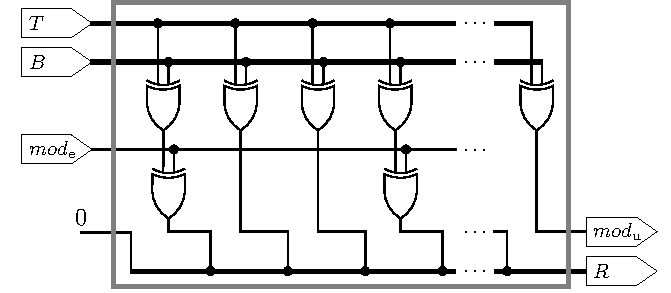
\includegraphics[width=12cm]{malu-optimized}
		\figcaption{MALU - Geoptimaliseerd ontwerp met shift}\label{figuur-implementatie-malu-optimized}
	\end{center}
\end{figure}

\section{Berekeningen in $\mathbb{F}_{2^m}$}\label{sectie-implementatie-gf2m}

\subsection{Basisontwerp}\label{subsectie-implementatie-gf2m-basisontwerp}

De eerder ontworpen MALU schakeling laat toe optellingen te doen, maar het Miller algoritme vereist dat er ook vermenigvuldigingen worden uitgerekend. Delingen en machtsverheffingen kunnen met behulp van vermenigvuldiging berekend worden en dienen dus niet rechtstreeks ge\"implementeerd te worden. Indien dus zowel optellingen als vermenigvuldigingen berekend kunnen worden, is alles voorhanden om de Tate pairing te berekenen.

Door toepassing van een ``shift and add'' algoritme, kan de waarde van \mbox{$A \cdot B = R$} berekend worden met behulp van de MALU schakeling. In \refalg{algoritme-implementatie-gf2m-multiply} is te zien hoe dit juist in z'n werk gaat. Door de modulo operatie telkens op het tussenresultaat uit te voeren, is het steeds van graad $\leq m$ en kan het opgeslagen worden in $T$. Op het einde moet het resultaat door $z$ gedeeld worden, wat neerkomt op een verschuiving van alle bits met 1 plaats naar rechts.

\begin{algorithm}[h]
\caption{``Shift and add'' vermenigvuldiging in $\mathbb{F}_{2^m}$}
\label{algoritme-implementatie-gf2m-multiply}
	\KwIn{$A, B \in \mathbb{F}_{2^m}/[P]$}
	\KwOut{$R \in \mathbb{F}_{2^m}/[P]$}
	\KwData{$T \in \mathbb{F}_{2^{m + 1}}$}
	\SetKwFunction{Degree}{Degree}

	$T \leftarrow 0$\;
	\For{$i \leftarrow m - 1$ \KwTo $0$}{
		\eIf{$A_i = 1$}{
			$b \leftarrow B$\;
		}{
			$b \leftarrow 0$\;
		}
	
		$T \leftarrow T \xor b$\;
	
		\If{$\Degree{T} = m$}{
			$T \leftarrow T \xor P$\;
		}
		$T \leftarrow T \ll 1$\;
	}
	$R \leftarrow T \gg 1$\;
\end{algorithm}

Wanneer de optelling en vermenigvuldiging nu in een schakeling gegoten worden, is het noodzakelijk een onderscheid te kunnen maken tussen beide bewerkingen. Ook moet kunnen aangegeven worden wanneer de berekening klaar is. Ten slotte moet het resultaat opgeslagen kunnen worden, zodat de uitgang van de schakeling correct blijft. Omdat in het Miller algoritme verscheidene keren de som $R + 1$ moet berekend worden, wordt ook een ingang $plus\_one$ voorzien. De uiteindelijke schakeling is te zien in \reffig{figuur-implementatie-wrapper-gf2m}. Het register $cycle$ is $\log _2 (m)$ bits groot en $T$ is $m$ bits. De waarde van $F_m$ wordt opgeslagen in register $mod$. Alle overige registers zijn 1 bit groot.

\begin{figure}[h]
	\begin{center}
		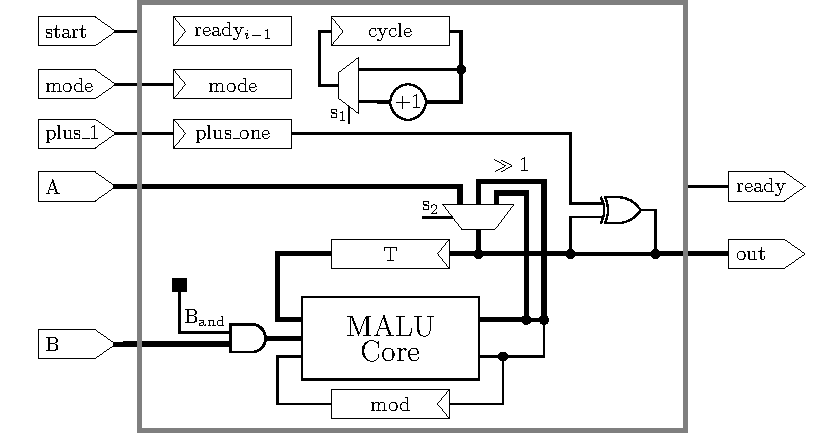
\includegraphics[width=12cm]{wrapper-gf2m}
		\figcaption{Schakeling voor berekeningen in $\mathbb{F}_{2^m}$}\label{figuur-implementatie-wrapper-gf2m}
	\end{center}
\end{figure}

Gezien de eenvoud van de schakeling is het niet nodig een FSM te implementeren, de besturing kan volledig via logica gebeuren. Die logica wordt getoond in \reffig{figuur-implementatie-wrapper-gf2m-logica}.

\begin{figure}[h]
	\begin{center}
		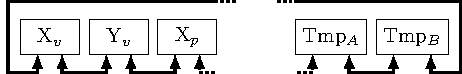
\includegraphics[width=12cm]{wrapper-gf2m-logica}
		\figcaption{Logica voor besturing van de schakeling voor berekeningen in $\mathbb{F}_{2^m}$}\label{figuur-implementatie-wrapper-gf2m-logica}
	\end{center}
\end{figure}

%Indien dit algoritme in een schakeling gegoten wordt, dienen enkele toevoegingen te gebeuren. Omdat een vermenigvuldiging langer dan \'e\'en klokslag duurt, is het noodzakelijk een $start$ ingang en $ready$ uitgang te hebben. Ook moet worden bijgehouden of $A$ en $B$ opgeteld of vermenigvuldigd dienen te worden. Deze functie wordt vervuld door het register $mode$. Ten slotte moet het mogelijk zijn om $R$ in $T$ op te slaan, zodat het juiste resultaat niet verloren gaat.

%Bij het hoog gaan van $start$, wordt nagegaan wat de waarde van $mode$ is. Indien het om een optelling gaat, wordt $A$ opgeslagen in $T$, anders wordt $T \leftarrow 0$ zoals in \refalg{algoritme-implementatie-gf2m-multiply}. Bij een optelling is het resultaat na \'e\'en klokslag beschikbaar aan de uitgang van het MALU blok. Het dient dan enkel nog 1 bit naar rechts verschoven te worden, net zoals moet gebeuren op het einde van een vermenigvuldiging.

%Wanneer dit alles in rekening gebracht wordt, verkrijgt men uiteindelijk de schakeling in \reffig{figuur-implementatie-wrapper-gf2m}. Om het geheel overzichtelijker te houden, bevat register $T$ een getal in $\mathbb{F}_{2^m}$ en wordt de waarde van $T_m$ bijgehouden in het register $mod$.

\subsection{Versnelling van de vermenigvuldiging}\label{subsectie-implementatie-gf2m-versnelling}

Wanneer met behulp van de schakeling in \reffig{figuur-implementatie-wrapper-gf2m} een vermenigvuldiging wordt berekend, zal het $m$ klokcycles duren eer het resultaat beschikbaar is aan de uitgang. Het is echter mogelijk dat aantal drastisch naar beneden te halen door $d$ MALU's te gebruiken en dus $d$ optellingen per klokcycle uit te voeren. Het principe hiervan wordt ge\"illustreerd in \reffig{figuur-implementatie-wrapper-gf2m-d}.

\begin{figure}[h]
	\begin{center}
		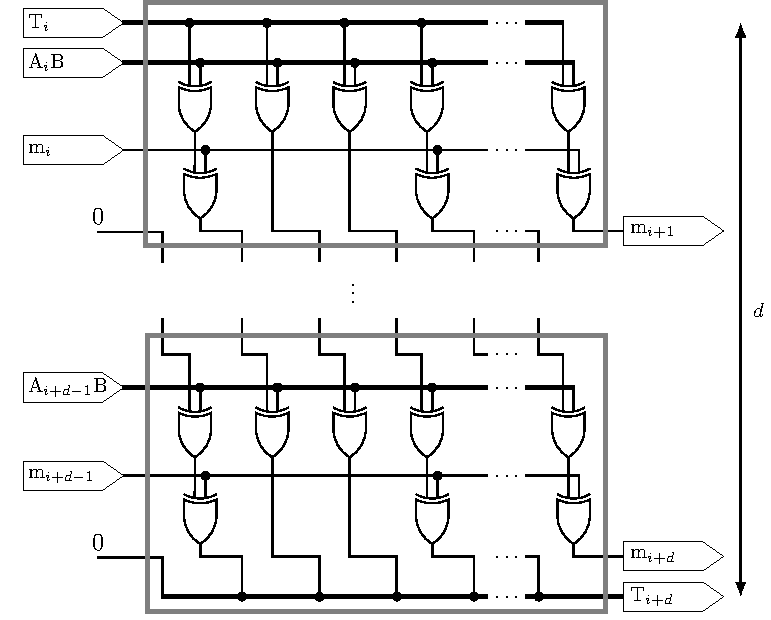
\includegraphics[width=12cm]{wrapper-gf2m-d}
		\figcaption{Schakeling voor berekeningen in $\mathbb{F}_{2^m}$ met woordbreedte $d$}\label{figuur-implementatie-wrapper-gf2m-d}
	\end{center}
\end{figure}

De rekentijd van het Miller algoritme zal door toepassing van deze techniek gevoelig verkort kunnen worden. Hoe groter $m$ en hoe meer vermenigvuldigigen er uitgevoerd dienen te worden, des te significanter de tijdswinst die geboekt kan worden. Uiteraard gaat het gebruik van deze techniek wel in tegen de eerder opgelegde beperking aan de grootte van de uiteindelijke schakeling. Het is echter niet zo dat er enkel $d - 1$ extra MALU blokken dienen toegevoegd te worden, afhankelijk van $d$ en $m$ dient ook een extra multiplexer in de schakeling gestoken te worden. Dit is zoals opgemerkt in \refsect{sectie-implementatie-beperkingen} een zeer slechte zaak voor de  oppervlakte.

Stel bijvoorbeeld $d = 4$ (en $m = 	163$). Het resultaat van een optelling zal net zoals in het standaard ontwerp aanwezig aan de uitgang van MALU \nr 1. Het resultaat van een vermenigvuldiging zal echter aan de uitgang van MALU \nr 3 verschijnen, aangezien $163 \bmod 4 = 3$. Het eindresultaat dat in $T$ dient opgeslagen te worden, is voor een vermenigvuldiging dus
\[T = mod3 \text{ \# } T3_{162:1}\]
, terwijl dit voor een optelling
\[T = mod1 \text{ \# } T1_{162:1}\]
is. Met andere woorden, er dient nu niet enkel gekozen te kunnen worden voor de ingang $A$, $T_{\text{out}}$ of $T1_{\text{ready}}$, maar ook voor $T3_{\text{ready}}$.

Indien men toch wenst het vermenigvuldigen te versnellen, is het aangeraden een $d$ te kiezen waarvoor
\[m \bmod d = 1\]

Als voorbeeld worden enkele voor de hand liggende en optimale keuzes vergeleken voor $d$ indien $m = 163$ in \reftbl{tabel-implementatie-woordbreedte-d}.

\begin{table}[h]
	\caption{Voor de hand liggende versus optimale waarden voor woordbreedte $d$ indien \mbox{$m=163$}}
	\label{tabel-implementatie-woordbreedte-d}
	\begin{tabular}{|l|c|c|c|c|c|c|}
		\hline
		\multicolumn{7}{|c|}{Voor de hand liggende waarden voor $d$}\\
		\hline
		$d$			& 2	& 4	& 8	& 16	& 32	& 64\\
		$m \bmod d$	& 1	& 3	& 3	& 3	& 3	& 35\\
		\hline
		\multicolumn{7}{c}{}\\
		\hline
		\multicolumn{7}{|c|}{Ideale waarden voor $d$}\\
		\hline
		$d$			& 2	& 3	& 6	& 9	& 18	& 27\\
		$m \bmod d$	& 1	& 1	& 1	& 1	& 1	& 1\\
		\hline
	\end{tabular}
\end{table}

\section{Controller voor het Miller algoritme}\label{sectie-implementatie-miller}


\subsection{Inleiding}\label{subsectie-implementatie-miller-inleiding}

Nu een schakeling voorhanden is die toelaat alle benodigde berekeningen uit te voeren, rest nog een schakeling te ontwerpen die het Miller algoritme (\refalg{algoritme-cryptografie-pairings-miller}) uitvoert. Het algoritme met invulling van de gekende parameters, zonder uitwerking van de berekeningen, wordt gegeven in \refalg{algoritme-implementatie-miller-algemeen}.

\begin{algorithm}[h]
	\caption{Miller algoritme voor berekening van de Tate pairing - Algemene versie}
	\label{algoritme-implementatie-miller-algemeen}
	\KwIn{$P, Q \in E(\mathbb{F}_{2^{163}})[l]$}
	\KwOut{e($P, Q$)}
	\KwData{$V \in E(\mathbb{F}_{2^{163}})[l]$; $F, G \in \mathbb{F}_{2^{4 \cdot 163}}$}
	$F \leftarrow 1$\;
	$V \leftarrow P$\;
	\For{$i \leftarrow 162$ \KwTo $0$}{
		$F \leftarrow F^2 \cdot G_{V,V}(\phi(Q))$\;\nllabel{lijn-implementatie-miller-algemeen-double-1}
		$V \leftarrow 2V$\;\nllabel{lijn-implementatie-miller-algemeen-double-2}
		\If{$i = 82$}{\nllabel{lijn-implementatie-miller-algemeen-add-if}
			$F \leftarrow F \cdot G_{V,P}(\phi(Q))$\;\nllabel{lijn-implementatie-miller-algemeen-add-1}
			$V \leftarrow V + P$\;\nllabel{lijn-implementatie-miller-algemeen-add-2}
		}
	}
	$F \leftarrow F^{\frac{2^{4 \cdot 163} - 1}{l}}$\;
	\KwRet{$F$}
\end{algorithm}

Merk op dat op lijn~\ref{lijn-implementatie-miller-algemeen-add-if} slechts \'e\'en waarde moet nagekeken worden, aangezien $l = 2^{163} + 2^{82} + 1$.

Om \refalg{algoritme-implementatie-miller-algemeen} te kunnen implementeren, moeten eerst de verschillende berekeningen uitgewerkt worden. Vervolgens zal aan de hand van die uitwerkingen bepaald worden welke registers de uiteindelijke schakeling ten minste nodig heeft en ten slotte zal een FSM ontworpen worden.

Grofweg kan het algoritme opgedeeld worden in de for-lus  en een finale exponentiatie. De for-lus kan verder onderverdeeld worden in een verdubbelingsstap, een optellingstap, een kwadratering van F en een vermenigvuldiging $F \cdot G$. Elk van deze stappen zal verder uitgediept worden en er zal voor elke berekening bepaald worden hoeveel tussenresultaten minimum opgeslagen moeten worden. Het zal blijken dat een inversie in $\mathbb{F}_{2^m}$ uitgerekend moet kunnen worden, wat ook verder uitgediept zal worden.

Bij elk van de volgende algoritmen zal aangegeven worden hoeveel en welke bewerkingen juist nodig zijn. Daarbij staat \textsf{A} voor een optelling, \textsf{M} voor een vermenigvuldiging, \textsf{S} voor een kwadratering en \textsf{I} voor een inversie. Aangezien er echter geen afzonderlijke schakeling voor kwadrateren ontworpen is, zijn \textsf{S} en \textsf{M} qua rekentijd in dit geval equivalent aan elkaar. De bewerking $a + 1$ neemt geen extra tijd in beslag, omdat die functie parallel met een optelling of vermenigvuldiging kan uitgevoerd worden door de $plus\_one$ van de schakeling voor berekeningen in $\mathbb{F}_{2^m}$ hoog te maken bij de start van een berekening.

\subsection{For-lus}\label{subsectie-implementatie-miller-forlus}

Zoals reeds eerder vermeld kan de for-lus onderverdeeld worden in een verdubbelingsstap, een optellingstap, een kwadratering van F en een vermenigvuldiging $F \cdot G$. Elk van deze onderdelen zal in de volgende paragrafen in detail aan bod komen.

\subsubsection{Verdubbelingsstap}

De verdubbelingstap wordt gevormd door lijnen \ref{lijn-implementatie-miller-algemeen-double-1} en \ref{lijn-implementatie-miller-algemeen-double-2} in \refalg{algoritme-implementatie-miller-algemeen}. Voor een hyperelliptische kromme zijn de berekeningen als volgt\cite{bertoni}:

\[\begin{aligned}
	\lambda &= x_V^2 + 1\\
	x_{2V} &= \lambda ^2\\
	y_{2V} &= \lambda (x_{2V} + x_V) + y_V + 1\\
	G_{V,V}(\phi(Q)) &= \lambda (x_{\phi} + x_V) + (y_{\phi} + y_V)\\
\end{aligned}\]

In dit geval kan $y_{2V}$ ook berekend worden als:

\[\begin{aligned}
y_{2V}	&= y_V^4 + x_V^4\\
			&= (y_V + x_V)^4\\	
\end{aligned}\]

Aangezien dit echter twee kwadrateringen en een optelling kost tegenover een vermenigvuldiging en twee optellingen, wordt de voorkeur gegeven aan de eerste methode.

Door de specifieke vorm van $\phi(Q)$ kan $G$ uitgeschreven worden als:

\[\begin{aligned}
	G_a	&=	\lambda (x_{\phi_a} + x_V) + (y_{\phi_a} + y_V)\qquad&
				G_c	&= \lambda \cdot x_{\phi_c} + y_{\phi_c}\\
	G_b	&=	\lambda \cdot x_{\phi_b} + y_{\phi_b}&
						&= 0\\
			&= \lambda + y_{\phi_b}&
				G_d	&= \lambda \cdot x_{\phi_d} + y_{\phi_d}\\
			&=	\lambda + x_{\phi_a}&
						&= 1\\
\end{aligned}\]

De variabele $G$ kan dus opgeslagen worden in twee registers van grootte $m$ in plaats van in vier. De vorm van $G$ zal ook toelaten de vermenigvuldiging $F \cdot G$ grotendeels te vereenvoudigen, zoals later gezien zal worden.

Wanneer dit in rekening gebracht wordt en het algoritme op register niveau wordt uitgeschreven, bekomt men uiteindelijk \refalg{algoritme-implementatie-miller-double-detail}. Hierbij werd specifiek gelet op een minimum gebruik van tijdelijke registers.

Buiten registers voor $x_{2V}$, $y_{2V}$, $x_{\phi_a}$, $y_{\phi_a}$, $G_a$ en $G_b$ is er ook een register nodig om $\lambda$ in op te slaan. In totaal moeten er zes optellingen, twee vermenigvuldigingen en twee kwadrateringen uitgerekend worden.

%Om te achterhalen in welke volgorde de bewerkingen best worden uitgevoerd om zo weinig mogelijk tussenresultaten te moeten opslaan. Het resultaat hiervan staat in \reftbl{tabel-implementatie-miller-double}. Een gearceerde cel betekend dat de aangeduide variabele op dat moment ingelezen moet worden. Indien er voor een variabele onder een bepaald niveau geen gearceerde cellen meer staan, kan deze verwijderd worden.

%\begin{minipage}[t]{10cm}
\begin{algorithm}[h]
	\caption{Uitwerking van de verdubbelingstap voor hyperelliptische krommen in het Miller algoritme}
	\label{algoritme-implementatie-miller-double-detail}
	\KwIn{$x_V, y_V \in E(\mathbb{F}_{2^m})$}
	\KwOut{$x_{2V}, y_{2V} \in E(\mathbb{F}_{2^m})$; $G \in \mathbb{F}_{2^{4m}}$}
	\KwData{$\lambda \in \mathbb{F}_{2^m}$}
	$G_a \leftarrow x_V$; $G_b \leftarrow y_V$\;
	$\lambda \leftarrow G_a^2 + 1$; $x_{2V} \leftarrow \lambda ^2$\comm{2 S}\;
	$y_{2V} \leftarrow x_{2V} + G_a$; $y_{2V} \leftarrow y_{2V} \cdot \lambda$\comm{1 M, 1 A}\;
	$y_{2V} \leftarrow y_{2V} + G_b + 1$\comm{1 A}\;
	$G_a \leftarrow G_a + x_{\phi_a}$; $G_a \leftarrow G_a \cdot \lambda$\comm{1 M, 1 A}\;
	$G_a \leftarrow G_a + y_{\phi_a}$; $G_a \leftarrow G_a + G_b$\comm{2 A}\;
	$G_b \leftarrow \lambda + x_{\phi_a}$\comm{1 A}\;
\end{algorithm}
%\end{minipage}
%\begin{minipage}[b]{3cm}
%	{\renewcommand{\arraystretch}{0.9}
%	\begin{tabular}{|c|c|c|}
%		\hline
%		$x_V$	& $y_V$	& $\lambda$\\
%		\hline
%		\shadecell & \shadecell & \\
%		& & \shadecell \\
%		& & \\
%		& & \shadecell \\
%		& & \\
%		& & \\
%		& & \shadecell \\
%		& & \\
%		& & \\
%		& & \shadecell \\
%		\hline
%	\end{tabular}}
%\end{minipage}

\subsubsection{Optellingstap}

De optellingstap bestaat uit lijnen \ref{lijn-implementatie-miller-algemeen-add-1} en \ref{lijn-implementatie-miller-algemeen-add-2} van \refalg{algoritme-implementatie-miller-algemeen}. Voor een hyperelliptische kromme dienen de volgende bewerkingen uitgevoerd te worden\cite{bertoni}:

\[\begin{aligned}
	\lambda &= \frac{y_V + y_P}{x_V + x_P}\\
	x_{V + P} &= \lambda ^2 + x_V + x_P\\
	y_{V + P} &= \lambda (x_{V+P} + x_P) + y_P + 1\\
	G_{V,V}(\phi(Q)) &= \lambda (x_{\phi} + x_P) + (y_{\phi} + y_P)\\
\end{aligned}\]

Net zoals bij de verdubbelingstap kan $G$ hier in 2 variabelen opgeslagen worden. Hoewel de optellingstap slechts \'e\'en maal moet worden uitgevoerd, is het uiteraard cruciaal dat ook hier zo weinig mogelijk tijdelijke variabelen gebruikt worden. Op die manier blijft de grootte van de uiteindelijke schakeling het kleinst. De uitgewerkte versie van het algoritme wordt gegeven in \refalg{algoritme-implementatie-miller-add-detail}.

In tegenstelling tot de verdubbelingstap zijn hier twee tijdelijke registers nodig, een voor $\lambda$ en een voor $a$. Verder zijn er twee registers nodig voor $x_P$ en $y_P$. Alles samen dienen er tien optellingen, drie vermenigvuldigingen, twee kwadrateringen en een inversie uitgerekend te worden.

\begin{algorithm}[h]
	\caption{Uitwerking van de optellingstap voor hyperelliptische krommen in het Miller algoritme}
	\label{algoritme-implementatie-miller-add-detail}
	\KwIn{$x_V, y_V, x_P, y_P \in E(\mathbb{F}_{2^m})$}
	\KwOut{$x_{V + P}, y_{V + P} \in E(\mathbb{F}_{2^m})$; $G \in \mathbb{F}_{2^{4m}}$}
	\KwData{$\lambda, a \in \mathbb{F}_{2^m}$}
	$G_a \leftarrow x_V$; $G_b \leftarrow y_V$\;
	$\lambda \leftarrow G_a + x_P$; $\lambda \leftarrow \lambda^{-1}$\comm{1 I, 1 A}\;
	$a \leftarrow G_b + y_P$; $\lambda \leftarrow \lambda \cdot a$\comm{1 M, 1 A}\;
	$x_{V + P} \leftarrow \lambda ^2 + G_a$; $x_{V + P} \leftarrow x_{V + P} + x_P$\comm{1 S, 2 A}\;
	$y_{V + P} \leftarrow x_{V + P} + x_P$; $y_{V + P} \leftarrow y_{V + P} \cdot \lambda$\comm{1 M, 1 A}\;
	$y_{V + P} \leftarrow y_{V + P} + y_P + 1$\comm{1 A}\;
	$G_a \leftarrow x_{\phi_a} + x_P$; $G_a \leftarrow G_a \cdot \lambda$\comm{1 M, 1 A}\;
	$G_a \leftarrow G_a + y_{\phi_a}$; $G_a \leftarrow G_a + y_P$\comm{2 A}\;
	$G_b \leftarrow \lambda + x_{\phi_a}$\comm{1 A}\;
\end{algorithm}

\subsubsection{Inversie}

De meest tijdrovende stap in de optellingstap is de inversie.  Zoals reeds vermeld in \refsect{sectie-cryptografie-gf}, kan een inversie in een Galois veld berekend worden door toepassing van Fermats kleine theorema:

\[\begin{aligned}
a^{2^m}		&= a\\
a^{2^m - 1}	&= 1\\
a^{2^m - 2}	&= a^{-1}\\
\end{aligned}\]

De naieve manier om dit te berekenen zou zijn om $a$ $2^m - 2$ keer met zichzelf te vermenigvuldigingen. In dit geval zou dat betekenen dat er $2^{163} -2 = 11 692 013 098 647 223 345 629 478 661 730 264 157 247 460 343 806$ vermenigvuldigingen zouden moeten uitgevoerd worden. Zoiets is uiteraard onhaalbaar.

Een tweede manier bestaat er in de exponent te ontbinden in machten van 2 en 3. In dat geval zouden er nog 237 vermenigvuldigen nodig zijn.

Er is echter een derde, optimale manier die toegepast kan worden indien de exponent van de vorm $2^m - 2$ is \cite{batina-pkc}\cite{itoh}. Dit gaat als volgt in zijn werk:

\[a^{2^m - 2} = (a^{2^{m - 1} - 1})^2\]

Als wordt aangenomen dat $m$ oneven is, is de macht van twee na het gelijkheidsteken dus even. Zolang de exponent even is, kan recursief volgende formule toegepast worden:

\[a^{2^i - 1} = (a^{2^{\frac{i}{2}} - 1})^{2^{\frac{i}{2}}} \cdot a^{2^{\frac{i}{2}} - 1}\]

Indien $a$ oneven is, dient volgende formule toegepast te worden:

\[a^{2^i - 1} = (a^{2^{i - 1} - 1})^2 \cdot a\]

Uiteindelijk eindigd men dan bij $a^2$ of $a^3$. Het totaal aantal bewerkingen voor een inversie in $\mathbb{F}_{2^m}$ is $\lfloor\log_2(m - 1)\rfloor + \text{Hamm}(m - 1) + 1$ vermenigvuldigingen en $m - 1$ kwadrateringen. $\text{Hamm}(x)$ staat daarbij voor het Hamming gewicht van de binaire voorstelling van $x$.

In het geval van $m = 163$ is de uiteindelijke keten van bewerkingen zoals gegeven in \refalg{algoritme-implementatie-miller-inversie}. Het aantal berekeningen in dat geval is 9 vermenigvuldigingen en 162 kwadrateringen. Er is een register nodig om $a$ bij de houden en twee voor de tussenresultaten $a^{2^i - 1}$ en $(a^{2^i - 1})^{2^i}$.

\begin{algorithm}[h]
	\caption{Inversie in $\mathbb{F}_{2^{163}}$}
	\label{algoritme-implementatie-miller-inversie}
	\KwIn{$a \in \mathbb{F}_{2^{163}}$}
	\KwOut{$a^{-1} \in \mathbb{F}_{2^{163}}$}
	$a^3 \leftarrow a^2 \cdot a$\comm{1 S, 1 M}\;
	$a^{2^4 - 1} \leftarrow (a^3)^{2^2} \cdot a^3$\comm{2 S, 1 M}\;
	$a^{2^5 - 1} \leftarrow (a^{2^4 - 1})^2 \cdot a$\comm{1 S, 1 M}\;
	$a^{2^{10} - 1} \leftarrow (a^{2^5 - 1})^{2^5} \cdot a^{2^5 - 1}$\comm{5 S, 1 M}\;
	$a^{2^{20} - 1} \leftarrow (a^{2^{10} - 1})^{2^{10}} \cdot a^{2^{10} - 1}$\comm{10 S, 1 M}\;
	$a^{2^{40} - 1} \leftarrow (a^{2^{20} - 1})^{2^{20}} \cdot a^{2^{20} - 1}$\comm{20 S, 1 M}\;
	$a^{2^{80} - 1} \leftarrow (a^{2^{40} - 1})^{2^{40}} \cdot a^{2^{40} - 1}$\comm{40 S, 1 M}\;
	$a^{2^{81} - 1} \leftarrow (a^{2^{80} - 1})^2 \cdot a$\comm{1 S, 1 M}\;
	$a^{2^{162} - 1} \leftarrow (a^{2^{81} - 1})^{2^{81}} \cdot a^{2^{81} - 1}$\comm{81 S, 1 M}\;
	$a^{-1} \leftarrow (a^{2^{162} - 1})^2$\comm{1 S}\;
\end{algorithm}

\subsubsection{Kwadratering van $F$}

Bij het uitvoeren van lijn~\ref{lijn-implementatie-miller-algemeen-double-1} van \refalg{algoritme-implementatie-miller-algemeen} moet ook telkens het kwadraat van $F$ berekend worden. De afleiding van de formule daarvoor gaat als volgt:

\[\begin{aligned}
F^2	&= (F_a + F_b x + F_c y + F_d xy) \cdot (F_a + F_b x + F_c y + F_d xy)\\
		&= F_a^2 + F_a F_b x + F_a F_c y + F_a F_d xy + F_b F_a x + F_b^2 x^2 + F_b F_c xy\\
			&\quad + F_b F_d x^2y + F_c F_a y + F_c F_b xy + F_c^2 y^2 + F_c F_d xy^2 + F_d F_a xy\\
			&\quad + F_d F_b x^2y + F_d F_c xy^2 + F_d^2 x^2 y^2\\
		&= (F_a^2 + F_b^2 + F_c^2 + F_d^2)\\
			&\quad + (F_a F_b + F_b F_a + F_b^2 + F_c F_d + F_d F_c + F_d^2)x\\
			&\quad + (F_a F_c + F_b F_d + F_c F_a + F_c^2 + F_c F_d + F_d F_b + F_d F_c)y\\
			&\quad + (F_a F_d + F_b F_c + F_b F_d + F_c F_b + F_c^2 + F_d F_a + F_d F_b + F_d^2)xy\\
		&= (F_a^2 + F_b^2 + F_c^2 + F_d^2) + (F_b^2 + F_d^2)x + F_c^2 y + (F_c^2 + F_d^2)xy\\
\end{aligned}\]

Het is mogelijk dit te berekenen zonder gebruik van tijdelijke variabelen. Er zijn dus enkel registers nodig voor $F_a$, $F_b$, $F_c$ en $F_d$. Hoe dat in z'n werk gaat is te zien in \refalg{algoritme-implementatie-miller-f-square}. E\'en kwadratering van $F$ vraagt vier optellingen en vier kwadrateringen.

\begin{algorithm}[h]
	\caption{Uitwerking van de kwadratering van $F$ in het Miller algoritme}
	\label{algoritme-implementatie-miller-f-square}
	\KwIn{$F \in \mathbb{F}_{2^{4m}}$}
	\KwOut{$F \in \mathbb{F}_{2^{4m}}$}
	$F_a \leftarrow F_a + F_c$\comm{1 A}\;
	$F_a \leftarrow F_a^2$\comm{1 S}\;
	$F_b \leftarrow F_b + F_d$\comm{1 A}\;
	$F_b \leftarrow F_b^2$\comm{1 S}\;
	$F_a \leftarrow F_a + F_b$\comm{1 A}\;
	$F_c \leftarrow F_c^2$\comm{1 S}\;
	$F_d \leftarrow F_d^2$\comm{1 S}\;
	$F_d \leftarrow F_d + F_c$\comm{1 A}\;
\end{algorithm}

\subsubsection{Vermenigvuldiging $F \cdot G$}

Zoals eerder opgemerkt, is $G$ in zowel de verdubbeling- als optellingstap niet van volledige rang in het extensieveld. De vermenigvuldiging van F met G kan daardoor vereenvoudigd worden, namelijk als volgt:

\[\begin{aligned}
F \cdot G	&= (F_a + F_b x + F_c y + F_d xy) \cdot (G_a + G_b x + xy)\\
	&= F_a G_a + F_a G_b x + F_a xy + F_b G_a x + F_b G_b x^2 + F_b x^2y + F_c G_a y\\
		&\quad + F_c G_b xy + F_c xy^2 + F_d G_a xy + F_d G_b x^2y + F_d x^2 y^2\\
	&= (F_a G_a + F_b G_b + F_d)\\
		&\quad + (F_a G_b + F_b G_a + F_b G_b + F_c + F_d)x\\
		&\quad + (F_b + F_c G_a + F_c + F_d G_b)y\\
		&\quad + (F_a + F_b + F_c G_b + F_d G_a + F_d G_b + F_d)xy\\
\end{aligned}\]

Indien hier nu de Karatsuba techniek op wordt toegepast, bekomt men:

\[\begin{aligned}
F \cdot G &= (F_a G_a + F_b G_b + F_d)\\
				&\quad + ((F_a + F_b) \cdot (G_a + G_b) + F_a G_a + F_c + F_d)x\\
				&\quad + (F_c G_a + F_d G_b + F_b + F_c)y\\
				&\quad + ((F_c + F_d) \cdot (G_a + G_b) + F_c G_a + F_a + F_b + F_d)xy\\
\end{aligned}\]

Deze formule kan uitgerekend wordt met gebruik van drie tijdelijke registers ($a$, $b$ en $c$). In totaal zijn er zes vermenigvuldigingen en veertien optellingen nodig. \refalg{algoritme-implementatie-miller-fg} beschrijft hoe de berekeningen juist gedaan moeten worden. Mist het gebruik van een vierde tijdelijk register zou het mogelijk zijn de berekening $G_a + G_b$ op te slaan. Die nu zowel in lijn~\ref{lijn-implementatie-miller-fg-gagb-1} als \ref{lijn-implementatie-miller-fg-gagb-2} berekend. Er zouden dan slechts dertien optellingen moeten berekend worden, \'e\'en minder dan \cite{beuchat}, waar $y^2 + y +x$ gebruikt wordt als modulo veelterm voor het extensieveld. Aangezien een extra tijdelijk register echter tegen de doelstellingen ingaat, wordt voor de iets langere berekening gekozen.

\begin{algorithm}[h]
	\caption{Uitwerking van de vermenigvuldiging $F \cdot G$ in het Miller algoritme}
	\label{algoritme-implementatie-miller-fg}
	\KwIn{$F, G \in \mathbb{F}_{2^{4m}}$}
	\KwOut{$F \in \mathbb{F}_{2^{4m}}$}
	\KwData{$a, b, c \in \mathbb{F}_{2^m}$}
	$a \leftarrow F_a \cdot G_a$; $a \leftarrow a + F_d$\comm{1 M, 1 A}\;
	$b \leftarrow F_a + F_b$; $c \leftarrow G_a + G_b$\comm{2 A}\;
	$b \leftarrow b \cdot c$; $b \leftarrow b + a$; $b \leftarrow b + F_c$\comm{1 M, 2 A}\;
	$c \leftarrow F_b \cdot G_b$; $a \leftarrow a + c$\comm{1 M, 1 A}\;
	$c \leftarrow F_c \cdot G_a$;	$c \leftarrow c + F_b$\comm{1 M, 1 A}\;
	$F_b \leftarrow b$; $b \leftarrow c$\;
	$c \leftarrow F_c + F_d$; $G_a \leftarrow G_a + G_b$\comm{2 A}\;
	$c \leftarrow c \cdot G_a$; $c \leftarrow c + b$; $c \leftarrow c + F_a$\comm{1 M, 2 A}\;
	$F_a \leftarrow a$\;
	$c \leftarrow c + F_d$; $b \leftarrow b + F_c$; $a \leftarrow F_d \cdot G_b$\comm{1 M, 2 A}\;
	$F_c \leftarrow b + a$; $F_d \leftarrow c$\comm{1 A}\;
\end{algorithm}

\subsection{Finale exponentiatie}\label{subsectie-implementatie-miller-finale-exp}

Eens de for-loop voltooid is, moet $F$ nog gereduceerd worden zodat het eindresultaat $e(P, Q)$ uniek is. Hoe dit gebeurt, wordt onderzocht in de volgende paragrafen

De reductie op het einde van het Miller algoritme bestaat uit de exponentiatie $e(P, Q) = F^M$, met

\[\begin{aligned}
M	&= \frac{2^{4m} - 1}{l}\\
	&= \frac{(2^{2m} + 1)(2^{2m} - 1)}{l}\\
	&= (2^{2m} - 1)(2^m - \nu 2^{\frac{m + 1}{2}} + 1)\\
	&= (2^{2m} - 1)(2^m + 1) + \nu(1 - 2^{2m})2^{\frac{m + 1}{2}}\\
\end{aligned}\]

De exponentiatie kan dus berekend worden als

\[e(P, Q) = \left(F^{2^{2m} - 1}\right)^{2^m + 1} \cdot \left(F^{1 - 2^{2m}}\right)^{2^{\frac{m + 1}{2}}}\]

Er zal onderzocht worden hoe elk van deze termen berekend kan worden. De methode uit \cite{beuchat} wordt hier aangepast aan het gekozen extensieveld. Stel $F = U_0 + U_1y$, met $U_0, U_1 \in \mathbb{F}_{2^{2m}}$. Met $y^{2^{2m}} = y + x + 1$ is $F^{2^{2m}} = U_0 + U_1 + U_1x + U_1y$. Men vindt dus 

\[\begin{aligned}
F^{2^{2m} - 1} = V &= \frac{U_0 + U_1 + U_1x + U_1y}{U_0 + U_1y}\\
	&= \frac{(U_0 + U_1 + U_1x + U_1y)^2}{(U_0 + U_1 + U_1x + U_1y) \cdot (U_0 + U_1y)}\\
%	&= \frac{U_0^2 + U_1^2 + U_1^2x + U_1^2y + U_1^2xy}{U_0^2 + U_1^2 + U_0 U_1 + U_0 U_1 x}\\
	&= \frac{U_0^2 + U_1^2 + U_1^2x}{U_0^2 + U_1^2 + U_0 U_1 + U_0 U_1 x} + \left[\frac{U_1^2 + U_1^2x}{U_0^2 + U_1^2 + U_0 U_1 + U_0 U_1 x}\right]y\\
\end{aligned}\]

en

\[\begin{aligned}
F^{1 - 2^{2m}}	= W &= \frac{U_0 + U_1y}{U_0 + U_1 + U_1x + U_1y}\\
	&= \frac{(U_0 + U_1y)^2}{(U_0 + U_1 + U_1x + U_1y) \cdot (U_0 + U_1y)}\\
%	&= \frac{U_0^2 + U_1^2 + + U_1^2y + U_1^2xy}{U_0^2 + U_1^2 + U_0 U_1 + U_0 U_1 x}\\
	&= \frac{U_0^2 + U_1^2}{U_0^2 + U_1^2 + U_0 U_1 + U_0 U_1 x} + \left[\frac{U_1^2 + U_1^2x}{U_0^2 + U_1^2 + U_0 U_1 + U_0 U_1 x}\right]y\\
\end{aligned}\]

Er moeten dus vier termen in $\mathbb{F}_{2^{2m}}$ berekend worden. Merk verder op dat de noemers van alle breuken in zowel $V$ als $W$ identiek zijn. Er zal dus slechts \'e\'en inversie in $\mathbb{F}_{2^{2m}}$ uitgerekend moeten worden. Ten slotte zijn de tweede termen van $V$ en $W$ identiek. Er moeten in totaal dus drie elementen in $\mathbb{F}_{2^{2m}}$ opgeslagen worden voor de uiteindelijke vermenigvuldiging van beide resultaten. Dit wil zeggen dat er dus zes registers van grootte $m$ nodig zijn.

Het kwadraat van een element $U \in \mathbb{F}_{2^{2m}}$ is

\[\begin{aligned}
U^2	&= u_0^2 + u_1^2 x^2\\
		&= (u_0^2 + u_1^2) + u_1^2 x\\
\end{aligned}\]


